% 例 1：菱形 AC=8, BD=6, 求面积与边长
\documentclass[tikz,border=4pt]{standalone}
\usepackage{ctex}
\usepackage{amsmath}
\usetikzlibrary{calc, decorations.markings}
\begin{document}
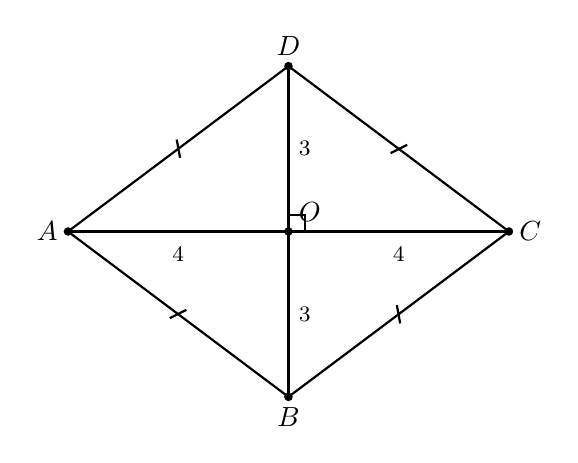
\begin{tikzpicture}[scale=0.7, thick,
  tickone/.style={postaction={decorate, decoration={markings,
    mark=at position 0.5 with {\draw (-1.5pt,-3pt) -- (1.5pt,3pt);}}}},
]
  \coordinate (A) at (-4,0);
  \coordinate (B) at (0,-3);
  \coordinate (C) at (4,0);
  \coordinate (D) at (0,3);
  \coordinate (O) at (0,0);
  \draw[tickone] (A) -- (B);
  \draw[tickone] (B) -- (C);
  \draw[tickone] (C) -- (D);
  \draw[tickone] (D) -- (A);
  \draw (A) -- (C);
  \draw (B) -- (D);
  % 直角
  \draw (0.3,0) -- (0.3,0.3) -- (0,0.3);
  \foreach \pt in {A,B,C,D,O} \filldraw (\pt) circle (1.6pt);
  \node[left]  at (A) {$A$};
  \node[below] at (B) {$B$};
  \node[right] at (C) {$C$};
  \node[above] at (D) {$D$};
  \node[above right] at (O) {$O$};
  \node[font=\footnotesize, below] at ($(A)!0.5!(O)+(0,-0.1)$) {$4$};
  \node[font=\footnotesize, below] at ($(O)!0.5!(C)+(0,-0.1)$) {$4$};
  \node[font=\footnotesize, right] at ($(O)!0.5!(D)$) {$3$};
  \node[font=\footnotesize, right] at ($(O)!0.5!(B)$) {$3$};
\end{tikzpicture}
\end{document}
